%! TEX program = pdflatex

\documentclass{beamer}

\usepackage{graphicx}
\usepackage[utf8x]{inputenc}
% \usepackage{hyperref}
% \usepackage{algorithm}
\usepackage{algorithmic}
% \usepackage{algpseudocode}  
\usepackage{algorithm2e}


\usetheme{Berkeley}

\title{
    Federated Learning Paper Sharing 
}
\author{
    Lisen Dai
}

\begin{document}
    \maketitle

    \section*{
        FedOpt (Appl. Sci. 2020, 10(8), 2864)
    }
    \begin{frame}
        \frametitle{
            \href{https://www.mdpi.com/2076-3417/10/8/2864}{
            FedOpt: Towards Communication Efficiency and Privacy Preservation in Federated Learning
            }
        }
        \framesubtitle{Sparse Compression Algorithm}
        Goal: reduce the number of communication bits during the models training. \\
        $$
        \Delta\theta = \mathcal{SGD}_n (\theta, D_{mini-batches}) - \theta
        $$
        $\theta$: Deep Neural Network parameters. \\
        $\mathcal{SGD}_n$: refers to the set of gradient updates after n epochs of SGD on DNN (deep neural network) parameters $\theta$ during the sampling of mini-batches from local data \\
        
        Once we have the updates $\delta v$... \\
        
    
    \end{frame}

    \begin{frame}
        \frametitle{
            \href{https://www.mdpi.com/2076-3417/10/8/2864}{
            FedOpt: Towards Communication Efficiency and Privacy Preservation in Federated Learning
            }
        }

        \begin{algorithm}[H]
            % \caption{SCA: Communication Efficiency in FedOpt}
            % \textbf{Initialisation:} \\
            % \textbf{Input:} temporal vector $\Delta \theta$, Sparsity Fraction $q$ \\
            % \textbf{Output:} : sparse temporal $\Delta \theta^*$ \\
      
            % \begin{algorithmic}[1]
            %     % \State{\textbf{Initialisation:}} \newline
            %     % $ num^+ \leftarrow top_{q}(\Delta \theta); num^- \leftarrow top_{q}(- \Delta \theta) $ \newline
            % \end{algorithmic}       
                        
            \KwIn{temporal vector $\Delta \theta$, Sparsity Fraction $q$}
            \KwOut{sparse temporal $\Delta \theta^*$}
            \caption{SCA: Communication Efficiency in FedOpt}
            \label{alg1}
            \textbf{Initialization}\;
            $ num^+ \leftarrow top_{q}(\Delta \theta); num^- \leftarrow top_{q}(- \Delta \theta) $ \\
            $ \Psi^+ \leftarrow mean(num^+); \Psi^- \leftarrow mean(num^-) $ \\
            \If{ $ \Psi^+ \geq \Psi^- $ }{
                \textbf{return} $ (\Delta \theta^* \leftarrow \Psi^+(\theta \geq \min(num^+))) $\;
            }
            \Else{
                \textbf{return} $ (- \Delta \theta^* \leftarrow \Psi^-(\theta \geq \min(-num^-))) $\;
            }
        \end{algorithm}
    
    \end{frame}

    \begin{frame}
        \frametitle{
            \href{https://www.mdpi.com/2076-3417/10/8/2864}{
            FedOpt: Towards Communication Efficiency and
            Privacy Preservation in Federated Learning
            }
        }
        
        \textit{\textbf{“We utilise the additively homomorphic encryption in FedOpt in order to achieve efficiency
        throughout the learning process.”}}

        \begin{figure}[H]
            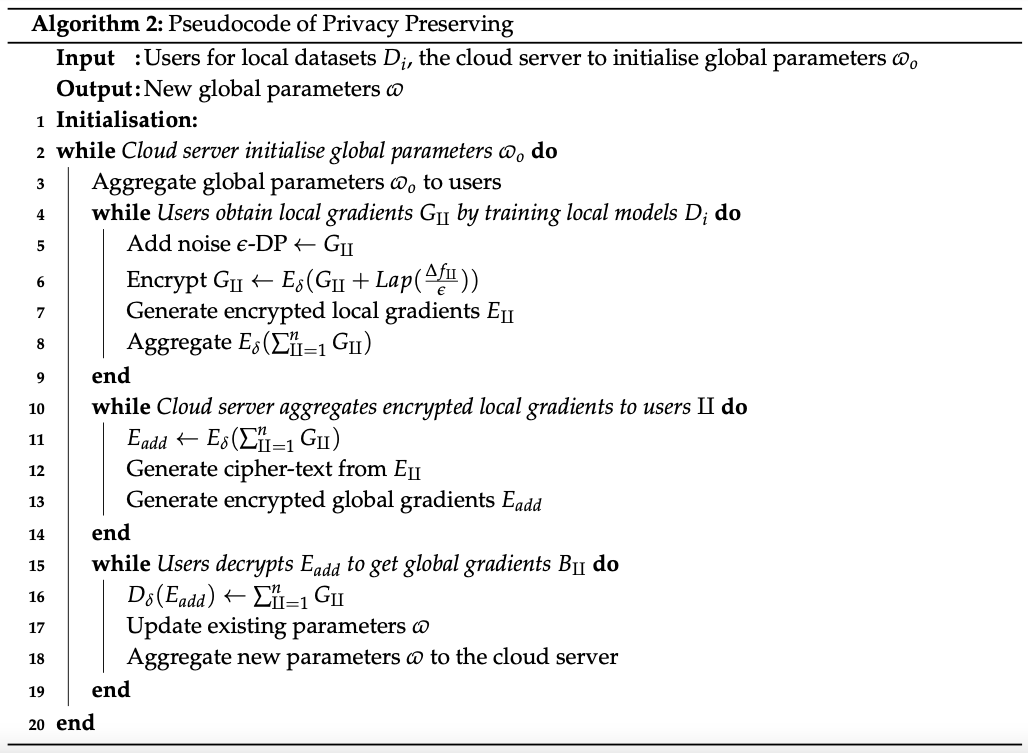
\includegraphics[width=0.8\textwidth]{src/Algorithm2.png}
        \end{figure}

    
    \end{frame}


    \begin{frame}
        \frametitle{
            \href{https://www.mdpi.com/2076-3417/10/8/2864}{
            FedOpt: Towards Communication Efficiency and
            Privacy Preservation in Federated Learning
            }
        }
        

        \begin{figure}[H]
            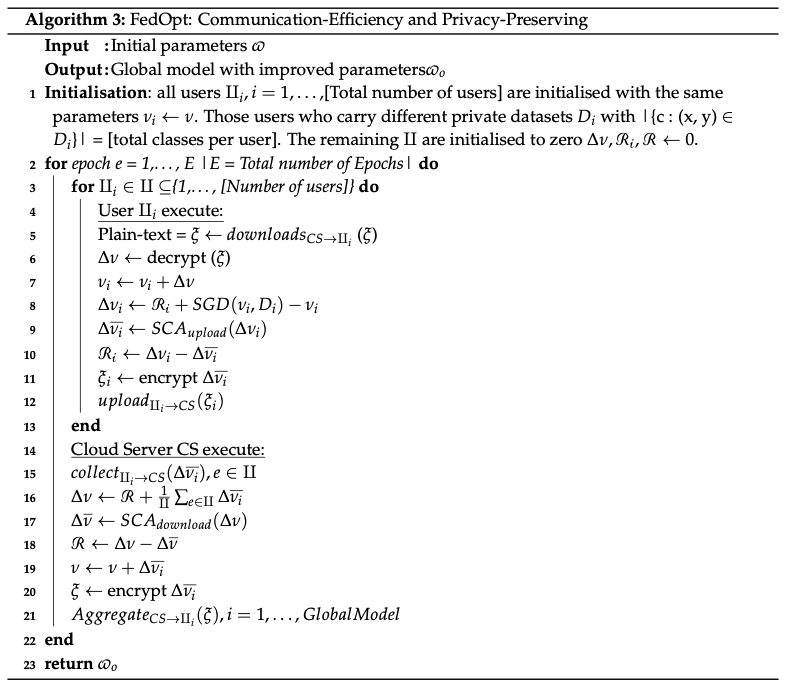
\includegraphics[width=0.8\textwidth]{src/Algorithm3.png}
        \end{figure}

    
    \end{frame}

    \begin{frame}
        \frametitle{
            \href{https://www.mdpi.com/2076-3417/10/8/2864}{
            FedOpt: Towards Communication Efficiency and
            Privacy Preservation in Federated Learning
            }
        }
        

        \begin{figure}[H]
            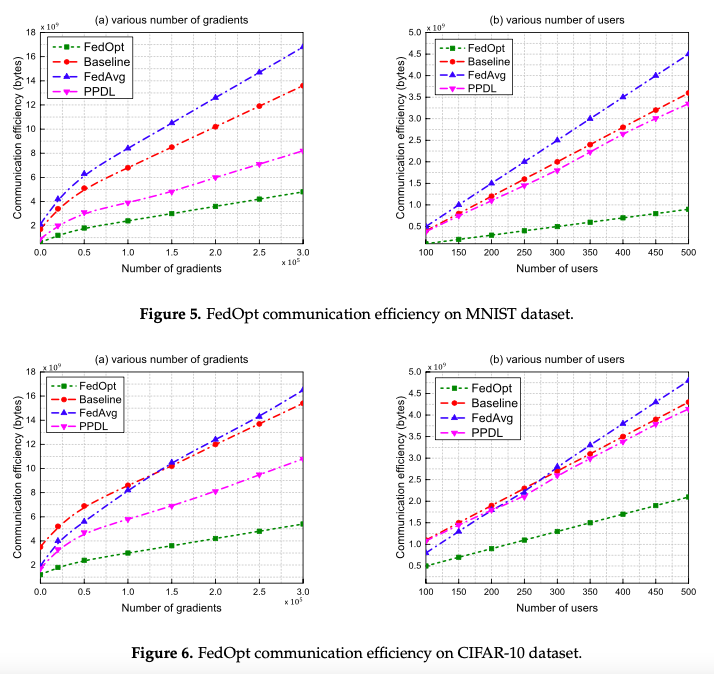
\includegraphics[width=0.8\textwidth]{src/Communication_Eff.png}
        \end{figure}

    
    \end{frame}

    \begin{frame}
        \frametitle{
            \href{https://www.mdpi.com/2076-3417/10/8/2864}{
            FedOpt: Towards Communication Efficiency and
            Privacy Preservation in Federated Learning
            }
        }
        

        \begin{figure}[H]
            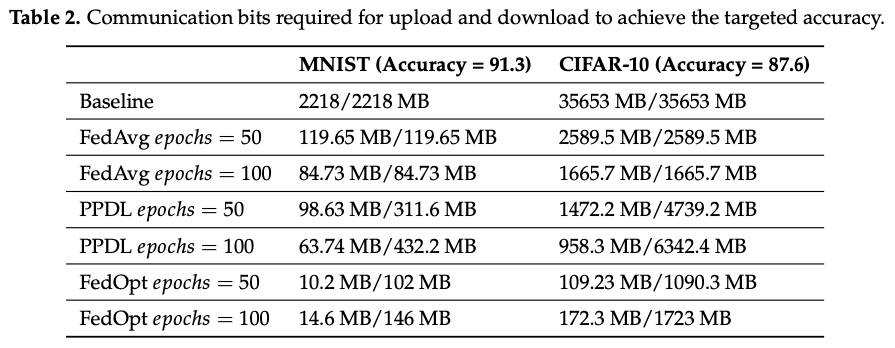
\includegraphics[width=\textwidth]{src/Accuracy.png}
        \end{figure}

    
    \end{frame}

\end{document}